\documentclass[12pt,a4paper]{article}
\usepackage[utf8]{inputenc}
\usepackage[T1]{fontenc}
\usepackage[english]{babel}
\usepackage{lmodern}
\usepackage{amsmath}
\usepackage{amssymb}
\usepackage{physics}
\usepackage{tcolorbox}
\usepackage{booktabs}
\usepackage{enumitem}
\usepackage[table,xcdraw]{xcolor}
\usepackage[left=2cm,right=2cm,top=2cm,bottom=2cm]{geometry}
\usepackage{pgfplots}
\pgfplotsset{compat=1.18}
\usepackage{graphicx}
\usepackage{float}
\usepackage{fancyhdr}
\usepackage{siunitx}
\usepackage{tikz}
\usepackage{adjustbox}
\usetikzlibrary{shapes.geometric}
\usepackage{hyperref} % Moved to last

% Custom Commands
\newcommand{\Tfield}{T(x)}
\newcommand{\alphaEM}{\alpha_{\text{EM}}}
\newcommand{\betaT}{\beta_{\text{T}}}
\newcommand{\Mpl}{M_{\text{Pl}}}
\newcommand{\Tzerot}{T_0(\Tfield)}
\newcommand{\e}{\mathrm{e}}
\newcommand{\alphaEMSI}{\alpha_{\text{EM,SI}}}

% Global Table Scaling Factor
\newcommand{\tablescale}{0.9}

% Header and Footer Configuration
\pagestyle{fancy}
\fancyhf{}
\fancyhead[L]{Johann Pascher}
\fancyhead[R]{Hierarchical Compilation of Units in the T0 Model}
\fancyfoot[C]{\thepage}
\renewcommand{\headrulewidth}{0.4pt}
\renewcommand{\footrulewidth}{0.4pt}

\hypersetup{
	colorlinks=true,
	linkcolor=blue,
	citecolor=blue,
	urlcolor=blue,
	pdftitle={Hierarchical Compilation of Units in the T0 Model with Energy as the Base Unit},
	pdfauthor={Johann Pascher},
	pdfsubject={Theoretical Physics},
	pdfkeywords={T0 Model, natural units, fine-structure constant, unified unit system, time-mass duality}
}

\begin{document}
	
	\title{Hierarchical Compilation of Units in the T0 Model with Energy as the Base Unit}
	\author{Johann Pascher}
	\date{April 13, 2025}
	
	\maketitle
	
	\begin{abstract}
		This work presents a comprehensive hierarchical compilation of natural units within the T0 model of time-mass duality, adopting energy as the fundamental unit. By normalizing dimensional constants (\(\hbar = c = G = k_B = 1\)) and dimensionless coupling constants (\(\alpha_{\text{EM}} = \alpha_W = \beta_T = 1\)) to unity, a unified framework emerges that integrates quantum, relativistic, and cosmological phenomena. The compilation details the hierarchy of constants, quantized length scales from sub-Planckian to cosmic regimes, and the unique presence of biological structures in forbidden zones. Electromagnetic, thermodynamic, and quantum mechanical constants are derived from the energy scale, with simplified field equations revealing the intrinsic unity of natural laws. The Einstein-Hilbert action underpins emergent gravitation, while precise conversions to SI units, philosophical implications, and experimental prospects enrich the discourse. Supported by extensive theoretical derivations and visualizations, this work offers a robust foundation for the T0 model, potentially advancing the unification of physics \cite{pascher_alphabeta_2025}.
	\end{abstract}
	
	\tableofcontents
	\newpage
	
	\section{Introduction}
	\label{sec:introduction}
	
	Natural units in theoretical physics streamline the description of physical laws by reducing independent dimensions and setting fundamental constants to unity, thereby unveiling the intrinsic simplicity underlying complex phenomena. Traditional systems, such as Planck units where \(\hbar = c = G = 1\), have long served as a cornerstone for theoretical explorations, eliminating arbitrary dimensional parameters and focusing on the essence of physical interactions \cite{Planck1899}. However, the T0 model of time-mass duality extends this paradigm by proposing a fully unified natural unit system, where not only dimensional constants (\(\hbar = c = G = k_B = 1\)) but also dimensionless coupling constants—the fine-structure constant \(\alpha_{\text{EM}}\), Wien’s constant \(\alpha_W\), and the model-specific T0 parameter \(\beta_T\)—are set to 1. This normalization is not a mere mathematical convenience but a profound theoretical necessity, reflecting the model’s premise that all physical laws converge into a singular, energy-based framework \cite{pascher_zeit_2025}.
	
	At its core, the T0 model redefines the fundamental relationship between time and mass, challenging conventional assumptions embedded in both relativity and quantum mechanics. In contrast to special relativity’s relative time or quantum mechanics’ treatment of time as a mere parameter, the T0 model posits time as an absolute entity, with mass varying dynamically in response to the system’s state. This conceptual inversion is mediated by the intrinsic time field, defined as:
	\[
	\Tfield = \frac{\hbar}{\max(m c^2, \omega)}
	\]
	This scalar field encapsulates the interplay between mass-energy and frequency, serving as a unifying bridge between the microscopic realm of quantum mechanics and the macroscopic domain of relativity. By reinterpreting gravitational effects as emergent phenomena arising from gradients in \(\Tfield\), the model eliminates the need for a fundamental gravitational interaction, aligning with modern theories of emergent gravity and offering a fresh perspective on cosmic dynamics \cite{Verlinde2011, pascher_emergente_2025}.
	
	The choice of energy as the base unit in the T0 model is both intuitive and revolutionary. Energy, as the common currency of physical interactions, allows all quantities—length, time, mass, temperature—to be expressed in terms of \([E]\) or its inverse \([E^{-1}]\), as detailed in Section \ref{sec:conversions}. This unification simplifies field equations, as shown in Section \ref{sec:field_equations}, and reveals hierarchical relationships among constants and scales, presented in Sections \ref{sec:hierarchy} and \ref{sec:length_scales}. The model’s ability to explain phenomena across scales—from quantum entanglement to cosmological redshift and dark energy—without invoking ad-hoc constructs like inflation or dark matter underscores its potential to reshape our understanding of the universe \cite{pascher_energiedynamik_2025}.
	
	This compilation aims to systematically present the natural units of the T0 model, emphasizing their definitions, values, and interconnections. It explores the theoretical foundations for setting \(\alpha_{\text{EM}} = \beta_T = 1\) (Section \ref{sec:derivations}), characterizes length scales spanning 97 orders of magnitude (Section \ref{sec:length_scales}), and highlights the surprising presence of biological structures in forbidden zones (Section \ref{sec:bio_anomalies}). The work further derives electromagnetic, thermodynamic, and quantum mechanical constants from the energy scale, presenting simplified field equations that illuminate the unity of natural laws (Section \ref{sec:field_equations}). The Einstein-Hilbert action provides a basis for emergent gravitation (Section \ref{sec:gravitation}), while conversions to SI units, philosophical implications, and experimental prospects enrich the discourse (Sections \ref{sec:conversions}, \ref{sec:philosophy}). Visualizations, such as Figures \ref{fig:length_hierarchy} and \ref{fig:quantity_network}, enhance clarity and interconnectedness.
	
	The objectives of this work are multifaceted:
	\begin{itemize}
		\item To delineate the hierarchical structure of fundamental constants and their values, as shown in Section \ref{sec:hierarchy}.
		\item To provide rigorous derivations for the normalization of \(\alpha_{\text{EM}}\) and \(\beta_T\), detailed in Section \ref{sec:derivations}.
		\item To characterize physical length scales and their quantization, including biological anomalies, as explored in Sections \ref{sec:length_scales} and \ref{sec:bio_anomalies}.
		\item To offer precise conversion formulas between natural and SI units, presented in Section \ref{sec:conversions}.
		\item To derive simplified field equations for electromagnetism, the T0 model, and quantum mechanics, analyzed in Section \ref{sec:field_equations}.
		\item To elucidate emergent gravitation via the Einstein-Hilbert action, compared with other theories in Section \ref{sec:gravitation}.
		\item To discuss philosophical implications, including ontological discreteness and emergent space-time, in Section \ref{sec:philosophy}.
		\item To propose experimental tests to validate the model’s predictions, outlined in Section \ref{sec:outlook} \cite{pascher_vereinheitlichung_2025}.
	\end{itemize}
	
	By weaving together these elements, this document seeks to provide a robust theoretical foundation for the T0 model, fostering a deeper understanding of the universe’s fundamental structure and paving the way for future explorations.
	
	\section{Part 1: Overview of Units and Scales}
	\label{sec:hierarchy}
	
	\subsection{Level 1: Primary Dimensional Constants}
	\label{subsec:level1}
	
	The T0 model’s natural unit system is anchored by dimensional constants set to unity, establishing the foundational scales of physics:
	\begin{itemize}
		\item \textbf{Reduced Planck Constant} (\(\hbar = 1\)): Defines the quantum scale, governing energy quantization, crucial for Section \ref{subsec:quantum} \cite{Planck1899}.
		\item \textbf{Speed of Light} (\(c = 1\)): Sets the relativistic scale, unifying space and time, essential for Section \ref{sec:gravitation} \cite{Einstein1905}.
		\item \textbf{Gravitational Constant} (\(G = 1\)): Establishes the gravitational scale, linked to emergent gravitation in Section \ref{sec:gravitation} \cite{Einstein1915}.
		\item \textbf{Boltzmann Constant} (\(k_B = 1\)): Defines the thermodynamic scale, connecting energy to temperature, supporting Section \ref{subsec:t0_equations}.
	\end{itemize}
	
	Dimensionless coupling constants, set to unity, govern interaction strengths:
	\begin{itemize}
		\item \textbf{Fine-Structure Constant} (\(\alpha_{\text{EM}} = 1\)): SI value \(\approx 1/137.036\), simplifies electromagnetic equations (Section \ref{subsec:maxwell}) \cite{pascher_alpha_2025}.
		\item \textbf{Wien’s Constant} (\(\alpha_W = 1\)): SI value \(\approx 2.82\), unifies thermodynamics.
		\item \textbf{T0 Parameter} (\(\beta_T = 1\)): SI value \(\approx 0.008\), central to \(\Tfield\) dynamics (Section \ref{subsec:beta_derivation}) \cite{pascher_beta_2025}.
	\end{itemize}
	
	These constants are summarized in Table \ref{tab:fund_const}, reflecting their role in the T0 model’s hierarchy.
	
	\begin{table}[htbp]
		\centering
		\begin{adjustbox}{width=\tablescale\textwidth}
			\begin{tabular}{llllll}
				\toprule
				\textbf{Constant} & \textbf{Symbol} & \textbf{SI Value} & \textbf{Natural Value} & \textbf{Derivation} & \textbf{Hierarchy Level} \\
				\midrule
				Reduced Planck Constant & \(\hbar\) & \(\SI{1.055e-34}{\joule\second}\) & 1 & Primary & Level 1 \\
				Speed of Light & \(c\) & \(\SI{3e8}{\meter\per\second}\) & 1 & Primary & Level 1 \\
				Gravitational Constant & \(G\) & \(\SI{6.674e-11}{\meter\cubed\per\kilogram\per\second\squared}\) & 1 & Primary & Level 1 \\
				Boltzmann Constant & \(k_B\) & \(\SI{1.381e-23}{\joule\per\kelvin}\) & 1 & Primary & Level 1 \\
				Fine-Structure Constant & \(\alpha_{\text{EM}}\) & 1/137.036 & 1 & Secondary & Level 2 \\
				Wien’s Constant & \(\alpha_W\) & 2.82 & 1 & Secondary & Level 2 \\
				T0 Parameter & \(\beta_T\) & 0.008 & 1 & Secondary & Level 2 \\
				\bottomrule
			\end{tabular}
		\end{adjustbox}
		\caption{Fundamental Constants in the T0 Model, linked to Sections \ref{subsec:alpha_derivation} and \ref{subsec:beta_derivation}}
		\label{tab:fund_const}
	\end{table}
	
	\subsection{Level 2.5: Derived Electromagnetic and Gravitational Constants}
	\label{subsec:level2.5}
	
	Derived constants emerge naturally with simplified values, reflecting the system’s coherence:
	\begin{itemize}
		\item \textbf{Vacuum Permeability} (\(\mu_0 = 1\)): Derived from \(\mu_0 = 1/(\varepsilon_0 c^2)\), simplifying electromagnetic equations (Section \ref{subsec:maxwell}).
		\item \textbf{Vacuum Permittivity} (\(\varepsilon_0 = 1\)): From \(\varepsilon_0 = 1/(\mu_0 c^2)\).
		\item \textbf{Vacuum Impedance} (\(Z_0 = 1\)): From \(Z_0 = \sqrt{\mu_0/\varepsilon_0}\).
		\item \textbf{Elementary Charge} (\(e = \sqrt{4\pi} \approx 3.544\)): From \(\alpha_{\text{EM}} = e^2/(4\pi \varepsilon_0 \hbar c) = 1\), making charge dimensionless, as discussed in Section \ref{subsec:alpha_derivation} \cite{Dirac1928}.
		\item \textbf{Planck Pressure} (\(p_P = 1\)): From \(p_P = c^7/(\hbar G^2)\).
		\item \textbf{Planck Force} (\(F_P = 1\)): From \(F_P = c^4/G\).
		\item \textbf{Einstein-Hilbert Action}:
		\[
		S_{\text{EH}} = \frac{1}{16\pi} \int R \sqrt{-g} \, d^4x
		\]
		Central to emergent gravitation, as elaborated in Section \ref{sec:gravitation} \cite{pascher_emergente_2025}.
	\end{itemize}
	
	These are summarized in Table \ref{tab:em_const}, illustrating their role in unifying physical interactions.
	
	\begin{table}[htbp]
		\centering
		\begin{adjustbox}{width=\tablescale\textwidth}
			\begin{tabular}{llllll}
				\toprule
				\textbf{Constant} & \textbf{Symbol} & \textbf{SI Value} & \textbf{Natural Value} & \textbf{Derivation} & \textbf{Hierarchy Level} \\
				\midrule
				Vacuum Permeability & \(\mu_0\) & \(\SI{1.256637061e-6}{\henry\per\meter}\) (\(4\pi \times 10^{-7}\)) & 1 & \(\mu_0 = 1/(\varepsilon_0 c^2)\) & Level 2.5 \\
				
				
				Vacuum Permittivity & \(\varepsilon_0\) & \(\SI{8.85e-12}{\farad\per\meter}\) & 1 & \(\varepsilon_0 = 1/(\mu_0 c^2)\) & Level 2.5 \\
				Vacuum Impedance & \(Z_0\) & \(\SI{376.73}{\ohm}\) & 1 & \(Z_0 = \sqrt{\mu_0/\varepsilon_0}\) & Level 2.5 \\
				Elementary Charge & \(e\) & \(\SI{1.602e-19}{\coulomb}\) & \(\sqrt{4\pi} \approx 3.544\) & \(e = \sqrt{4\pi \varepsilon_0 \hbar c}\) & Level 2.5 \\
				Planck Pressure & \(p_P\) & \(\SI{4.63e113}{\pascal}\) & 1 & \(p_P = c^7/(\hbar G^2)\) & Level 2.5 \\
				Planck Force & \(F_P\) & \(\SI{1.21e44}{\newton}\) & 1 & \(F_P = c^4/G\) & Level 2.5 \\
				\bottomrule
			\end{tabular}
		\end{adjustbox}
		\caption{Derived Electromagnetic and Gravitational Constants in the T0 Model, linked to Sections \ref{subsec:alpha_derivation}, \ref{subsec:maxwell}, and \ref{sec:gravitation}}
		\label{tab:em_const}
	\end{table}
	
	\subsection{Planck Units in the T0 Model}
	\label{subsec:planck_units}
	
	Planck units, derived from \(\hbar\), \(c\), and \(G\), are normalized to 1, as shown in Table \ref{tab:planck_units}. They serve as reference points for all scales, facilitating conversions (Section \ref{sec:conversions}) and anchoring the hierarchy in Figure \ref{fig:length_hierarchy} \cite{pascher_planck_2025}.
	
	\begin{table}[htbp]
		\centering
		\begin{adjustbox}{width=\tablescale\textwidth}
			\begin{tabular}{lcccl}
				\toprule
				\textbf{Planck Unit} & \textbf{Symbol} & \textbf{Definition} & \textbf{SI Value} & \textbf{Significance} \\
				\midrule
				Planck Length & \(l_P\) & \(\sqrt{\hbar G/c^3}\) & \(\SI{1.616e-35}{\meter}\) & Length unit \\
				Planck Time & \(t_P\) & \(\sqrt{\hbar G/c^5}\) & \(\SI{5.391e-44}{\second}\) & Time unit \\
				Planck Mass & \(m_P\) & \(\sqrt{\hbar c/G}\) & \(\SI{2.176e-8}{\kilogram}\) & Mass unit \\
				Planck Energy & \(E_P\) & \(\sqrt{\hbar c^5/G}\) & \(\SI{1.956e9}{\joule}\) & Energy unit \\
				Planck Temperature & \(T_P\) & \(\sqrt{\hbar c^5/G}/k_B\) & \(\SI{1.417e32}{\kelvin}\) & Temperature unit \\
				Planck Charge & \(q_P\) & \(\sqrt{4\pi \varepsilon_0 \hbar c}\) & \(\SI{1.875e-18}{\coulomb}\) & Charge unit \\
				Planck Pressure & \(p_P\) & \(c^7/(\hbar G^2)\) & \(\SI{4.633e113}{\pascal}\) & Pressure unit \\
				Planck Density & \(\rho_P\) & \(c^5/(\hbar G^2)\) & \(\SI{5.155e96}{\kilogram\per\meter\cubed}\) & Density unit \\
				\bottomrule
			\end{tabular}
		\end{adjustbox}
		\caption{Planck Units in the T0 Model}
		\label{tab:planck_units}
	\end{table}
	
	\subsection{Characteristic Length Scales}
	\label{sec:length_scales}
	
	The T0 model organizes length scales hierarchically, as detailed in Table \ref{tab:length_scales}, spanning from the Planck length (\(l_P\)) to the cosmological correlation length (\(L_T\)). This hierarchy, visualized in Figure \ref{fig:length_hierarchy}, covers 97 orders of magnitude, with each scale linked to specific physical phenomena, as discussed in Section \ref{subsec:quantization}.
	
	\begin{table}[H]
		\centering
		\begin{adjustbox}{width=\tablescale\textwidth}
			\begin{tabular}{lccc}
				\toprule
				\textbf{Structure} & \textbf{With \(l_P = 1\)} & \textbf{With \(r_0 = 1\)} & \textbf{Relationship} \\
				\midrule
				Planck Length (\(l_P\)) & 1 & \(1/\xi \approx 7519\) & Base unit \\
				T0 Length (\(r_0\)) & \(\xi \approx 1.33 \times 10^{-4}\) & 1 & \(\xi \cdot l_P\) \\
				Strong Scale & \(\sim 10^{-19}\) & \(\sim 10^{-15}\) & \(\sim \alpha_s \cdot \lambda_{C,h}\) \\
				Higgs Length (\(\lambda_{C,h}\)) & \(\sim 1.6 \times 10^{-20}\) & \(\sim 1.2 \times 10^{-16}\) & \(m_P/m_h \cdot l_P\) \\
				Proton Radius & \(\sim 5.2 \times 10^{-20}\) & \(\sim 3.9 \times 10^{-16}\) & \(\sim \alpha_s/(2\pi) \cdot \lambda_{C,p}\) \\
				Electron Radius (\(r_e\)) & \(\sim 2.4 \times 10^{-23}\) & \(\sim 1.8 \times 10^{-19}\) & \(\alphaEMSI/(2\pi) \cdot \lambda_{C,e}\) \\
				Compton Length (\(\lambda_{C,e}\)) & \(\sim 2.1 \times 10^{-23}\) & \(\sim 1.6 \times 10^{-19}\) & \(m_P/m_e \cdot l_P\) \\
				Bohr Radius (\(a_0\)) & \(\sim 2.9 \times 10^{-21}\) & \(\sim 2.2 \times 10^{-17}\) & \(\lambda_{C,e}/\alphaEMSI\) \\
				DNA Width & \(\sim 1.2 \times 10^{-26}\) & \(\sim 9.0 \times 10^{-23}\) & \(\sim \lambda_{C,e} \cdot m_e/m_{\text{DNA}}\) \\
				Cell & \(\sim 6.2 \times 10^{-30}\) & \(\sim 4.7 \times 10^{-26}\) & \(\sim 10^7 \cdot \text{DNA}\) \\
				Human & \(\sim 6.2 \times 10^{-35}\) & \(\sim 4.7 \times 10^{-31}\) & \(\sim 10^5 \cdot \text{Cell}\) \\
				Earth Radius & \(\sim 3.9 \times 10^{-41}\) & \(\sim 2.9 \times 10^{-37}\) & \(\sim (m_P/m_{\text{Earth}})^2 \cdot l_P\) \\
				Sun Radius & \(\sim 4.3 \times 10^{-43}\) & \(\sim 3.2 \times 10^{-39}\) & \(\sim (m_P/m_{\text{Sun}})^2 \cdot l_P\) \\
				Solar System & \(\sim 6.2 \times 10^{-47}\) & \(\sim 4.7 \times 10^{-43}\) & \(\sim \alpha_G^{-1/2} \cdot \text{Sun}\) \\
				Galaxy & \(\sim 6.2 \times 10^{-56}\) & \(\sim 4.7 \times 10^{-52}\) & \(\sim (m_P/m_{\text{Galaxy}})^2 \cdot l_P\) \\
				Cluster & \(\sim 6.2 \times 10^{-58}\) & \(\sim 4.7 \times 10^{-54}\) & \(\sim 10^2 \cdot \text{Galaxy}\) \\
				Horizon (\(d_H\)) & \(\sim 5.4 \times 10^{61}\) & \(\sim 4.1 \times 10^{65}\) & \(\sim 1/H_0\) \\
				Correlation Length (\(L_T\)) & \(\sim 3.9 \times 10^{62}\) & \(\sim 2.9 \times 10^{66}\) & \(\sim \betaT^{-1/4} \cdot \xi^{-1/2} \cdot l_P\) \\
				\bottomrule
			\end{tabular}
		\end{adjustbox}
		\caption{Length Scales}
		\label{tab:length_scales}
	\end{table}
	
	\begin{figure}[htbp]
		\centering
		\begin{tikzpicture}
			\small
			\draw[thick,->] (0,0) -- (12,0) node[right] {$\log(L/l_P)$};
			\draw[thick,->] (0,0) -- (0,5) node[above] {Energy Scale};
			\draw (0,0.2) -- (0,-0.2) node[below] {$0$};
			\draw (1,0.2) -- (1,-0.2) node[below] {$r_0$};
			\draw (5,0.2) -- (5,-0.2) node[below] {$\lambda_{C,e}$};
			\draw (6,0.2) -- (6,-0.2) node[below] {$a_0$};
			\draw (11,0.2) -- (11,-0.2) node[below] {$L_T$};
			\node[blue] at (0,1.2) {$l_P = 1$};
			\node[blue] at (1,1.7) {$r_0 \approx 10^{-4}$};
			\node[blue] at (5,1.7) {$\lambda_{C,e} \approx 10^{-23}$};
			\node[blue] at (6,1.2) {$a_0 \approx 2.9 \times 10^{-21}$};
			\node[blue] at (11,1.2) {$L_T \approx 10^{62}$};
			\draw [decorate,decoration={brace,amplitude=10pt,mirror},xshift=0pt,yshift=-20pt]
			(0,0) -- (1,0) node [black,midway,yshift=-20pt] {Primordial Scale};
			\draw [decorate,decoration={brace,amplitude=10pt,mirror},xshift=0pt,yshift=-20pt]
			(4.8,0) -- (6.2,0) node [black,midway,yshift=-20pt] {Quantum Scale};
			\draw [decorate,decoration={brace,amplitude=10pt,mirror},xshift=0pt,yshift=-20pt]
			(10.8,0) -- (12,0) node [black,midway,yshift=-20pt] {Cosmological Scale};
			\draw[dashed, red] (1,0.5) -- (5,0.5) node[midway, above] {$\propto m_h/m_e$};
			\draw[dashed, red] (6,0.5) -- (11,0.5) node[midway, above] {$\propto 1/H_0$};
		\end{tikzpicture}
		\caption{Hierarchy of length scales in the T0 model, spanning from \(r_0\) to \(L_T\), covering 66 orders of magnitude, as detailed in Section \ref{subsec:quantization}.}
		\label{fig:length_hierarchy}
	\end{figure}
	
	\subsection{Biological Anomalies in Forbidden Zones}
	\label{sec:bio_anomalies}
	
	A striking feature of the T0 model is the presence of biological structures in “forbidden zones” between quantized scales, as shown in Table \ref{tab:bio_anomalies} and Figure \ref{fig:stability_zones}. These zones, discussed in Section \ref{subsec:quantization}, lack stable physical structures, yet biological systems thrive due to unique stabilization mechanisms:
	\[
	\nabla^2 \Tfield_{\text{bio}} \approx -\frac{\rho}{\Tfield^2} + \delta_{\text{bio}}(x,t)
	\]
	The term \(\delta_{\text{bio}}\) accounts for information-based, topological, and dynamic stabilization, distinguishing life from inanimate matter \cite{pascher_dualismus_2025}.
	
	The forbidden zones, spanning approximately 19 and 3 orders of magnitude, represent regions where stable physical structures are absent due to the quantization of length scales. The ~19-order gap, between \( r_0 \approx 1.33 \times 10^{-4} l_P \) and \( \lambda_{C,e} \approx 2.1 \times 10^{-23} l_P \), arises from the mass ratio \( m_h / m_e \approx 2.45 \times 10^{17} \), leading to a logarithmic separation of \( \log(m_h / m_e) \approx 19.39 \). The ~3-order gap, between \( \lambda_{C,e} \approx 2.1 \times 10^{-23} l_P \) and \( a_0 \approx 2.9 \times 10^{-21} l_P \), corresponds to the fine-structure constant \( \alpha_{\text{EM,SI}} \approx 1/137.036 \), with \( \log(1 / \alpha_{\text{EM,SI}}) \approx 2.14 \), approximated as ~3 for simplicity. These gaps are computed as:
	\[
	\Delta \log(L / l_P) = \log\left(\frac{L_2}{L_1}\right)
	\]
	where \( L_1 \) and \( L_2 \) are adjacent quantized scales. Biological structures, such as DNA and cells, occupy these zones due to dynamic stabilization mechanisms, as discussed in Section \ref{subsec:quantization}.
	
	\begin{table}[htbp]
		\centering
		\begin{adjustbox}{width=\tablescale\textwidth}
			\begin{tabular}{lccc}
				\toprule
				\textbf{Structure} & \textbf{Size} & \textbf{Ratio to \(l_P\)} & \textbf{Position} \\
				\midrule
				DNA Diameter & \(\SI{2e-9}{\meter}\) & \(\sim 10^{-26}\) & Forbidden Zone \\
				Protein & \(\SI{1e-8}{\meter}\) & \(\sim 10^{-27}\) & Forbidden Zone \\
				Bacterium & \(\SI{1e-6}{\meter}\) & \(\sim 10^{-29}\) & Forbidden Zone \\
				Cell & \(\SI{1e-5}{\meter}\) & \(\sim 10^{-30}\) & Forbidden Zone \\
				Organism & \(\SIrange{1e-3}{1}{\meter}\) & \(\sim 10^{-32} - 10^{-35}\) & Forbidden Zone \\
				\bottomrule
			\end{tabular}
		\end{adjustbox}
		\caption{Biological Structures in Forbidden Zones, as visualized in Figure \ref{fig:stability_zones}}
		\label{tab:bio_anomalies}
	\end{table}
	
	\section{Part 2: Detailed Explanations and Derivations}
	\label{sec:derivations}
	
	\subsection{Fundamental Concepts of the T0 Model}
	\label{subsec:concepts}
	
	The T0 model redefines the interplay between time and mass, positing time as an absolute entity and mass as a variable quantity, challenging the paradigms of relativity (relative time, constant mass) and quantum mechanics (parametric time). This shift is facilitated by the intrinsic time field:
	\[
	\Tfield = \frac{\hbar}{\max(m c^2, \omega)}
	\]
	This scalar field encapsulates the dynamic relationship between mass-energy and frequency, acting as a mediator that unifies quantum and relativistic phenomena. By treating time as absolute, the model reinterprets relativistic effects—such as time dilation—as variations in mass, offering a novel perspective on phenomena like gravitational redshift and particle interactions \cite{pascher_zeit_2025}.
	
	The normalization of constants (\(\hbar = c = G = k_B = \alpha_{\text{EM}} = \alpha_W = \beta_T = 1\)) is a theoretical necessity, reflecting the model’s premise that physical laws are inherently unified. Energy, as the base unit, allows all quantities to be expressed in a consistent dimensional framework, as shown in Table \ref{tab:practical_notation}. Gravitation emerges from \(\Tfield\) gradients, eliminating the need for a fundamental gravitational force, as detailed in Section \ref{sec:gravitation}. This unification bridges micro- and macro-scales, explaining phenomena from quantum entanglement to cosmic expansion without ad-hoc assumptions \cite{pascher_emergente_2025}.
	
	\subsection{Derivation of \(\beta_T = 1\)}
	\label{subsec:beta_derivation}
	
	The T0 parameter \(\beta_T\), governing the coupling of \(\Tfield\), is normalized to 1 through a rigorous derivation linked to Standard Model parameters:
	\[
	\betaT = \frac{\lambda_h^2 v^2}{16 \pi^3} \cdot \frac{1}{m_h^2} \cdot \frac{1}{\xi}
	\]
	where:
	\begin{itemize}
		\item \(\lambda_h \approx 0.13\): Higgs self-coupling.
		\item \(v \approx \SI{246}{\giga\electronvolt}\): Higgs vacuum expectation value.
		\item \(m_h \approx \SI{125}{\giga\electronvolt}\): Higgs mass.
		\item \(\xi = r_0/l_P\): T0 length to Planck length ratio, as shown in Table \ref{tab:length_scales}.
	\end{itemize}
	
	Setting \(\betaT = 1\):
	\[
	\xi = \frac{\lambda_h^2 v^2}{16 \pi^3 m_h^2} \approx 1.33 \times 10^{-4}
	\]
	This yields \(r_0 \approx 1.33 \times 10^{-4} \cdot l_P\). Using \(m_h^2 = 2 \lambda_h v^2\):
	\[
	\xi = \frac{\lambda_h}{32 \pi^3} \approx 1.31 \times 10^{-4}
	\]
	The consistency of these values validates the derivation, as visualized in Figure \ref{fig:energy_hierarchy}. \(\beta_T = 1\) acts as a renormalization fixed point:
	\[
	\lim_{E \to 0} \betaT(E) = 1
	\]
	The SI value \(\betaT \approx 0.008\) reflects finite-energy effects, reinforcing the model’s coherence \cite{pascher_beta_2025}.
	
	\subsection{Derivation of \(\alpha_{\text{EM}} = 1\)}
	\label{subsec:alpha_derivation}
	
	The fine-structure constant’s normalization is pivotal for electromagnetism:
	\[
	\alphaEM = \frac{e^2}{4 \pi \varepsilon_0 \hbar c} \approx \frac{1}{137.036}
	\]
	With \(\hbar = c = \varepsilon_0 = 1\), setting \(\alphaEM = 1\):
	\[
	e^2 = 4 \pi \implies e = \sqrt{4 \pi} \approx 3.544
	\]
	This makes charge dimensionless, simplifying equations in Section \ref{subsec:maxwell}. Alternatively, using the classical electron radius \(r_e = e^2/(4 \pi \varepsilon_0 m_e c^2)\) and Compton wavelength \(\lambda_C = h/(m_e c)\):
	\[
	\alphaEM = \frac{2 \pi r_e}{\lambda_C}
	\]
	With \(h = 2 \pi \hbar\), this confirms the standard definition \cite{pascher_alpha_2025}. The coupling of \(\mu_0\) and \(\varepsilon_0\):
	\[
	\mu_0 \varepsilon_0 = \frac{1}{c^2} = 1
	\]
	unifies electromagnetic interactions, as shown in Table \ref{tab:em_const} \cite{pascher_alphabeta_2025}. The Bohr radius is defined consistently as:
	\[
	a_0 = \frac{\lambda_{C,e}}{\alpha_{\text{EM,SI}}} \approx 2.9 \times 10^{-21} l_P
	\]
	
	\subsection{Connection to Higgs Parameters}
	\label{subsec:higgs}
	
	The T0 length \(r_0\) links directly to Standard Model parameters:
	\[
	r_0 = \xi \cdot l_P = \frac{\lambda_h^2 v^2}{16 \pi^3 m_h^2} \cdot l_P \approx 1.33 \times 10^{-4} \cdot l_P
	\]
	With \(m_h^2 = 2 \lambda_h v^2\):
	\[
	\xi = \frac{\lambda_h}{32 \pi^3} \approx 1.31 \times 10^{-4}
	\]
	This connection, visualized in Figure \ref{fig:energy_hierarchy}, bridges quantum field theory and emergent gravitation, reinforcing the model’s coherence across scales, as discussed in Section \ref{sec:length_scales} \cite{pascher_higgs_2025}.
	
	\subsection{Quantization of Length Scales}
	\label{subsec:quantization}
	
	The T0 model reveals a discrete hierarchy of length scales, analogous to atomic energy levels, as shown in Table \ref{tab:length_scales} and Figure \ref{fig:length_hierarchy}. This quantization, a cornerstone of the model, follows:
	\[
	L_n = l_P \times \prod_i \alpha_i^{n_i}
	\]
	where \(\alpha_i = \{\alpha_{\text{EM}}, \beta_T, \xi\}\) and \(n_i\) are quantum numbers. Key scales include:
	\begin{itemize}
		\item \textbf{Planck Length}: \(L_n = l_P\), \(n_i = 0\).
		\item \textbf{T0 Length}: \(r_0 = \xi \cdot l_P\), \(n_\xi = 1\).
		\item \textbf{Compton Wavelength}: \(\lambda_{C,e} \approx 10^{-23} l_P\), linked to electron dynamics (Section \ref{subsec:quantum}).
		\item \textbf{Bohr Radius}: \(a_0 = \lambda_{C,e} / \alpha_{\text{EM,SI}} \approx 2.9 \times 10^{-21} l_P\), defining atomic structures.
		\item \textbf{Correlation Length}: \(L_T \approx 10^{62} l_P\), marking the cosmic horizon \cite{pascher_planck_2025}.
	\end{itemize}
	
	\par % Ensure outer paragraph mode
	
	\begin{figure}[htbp]
		\centering
		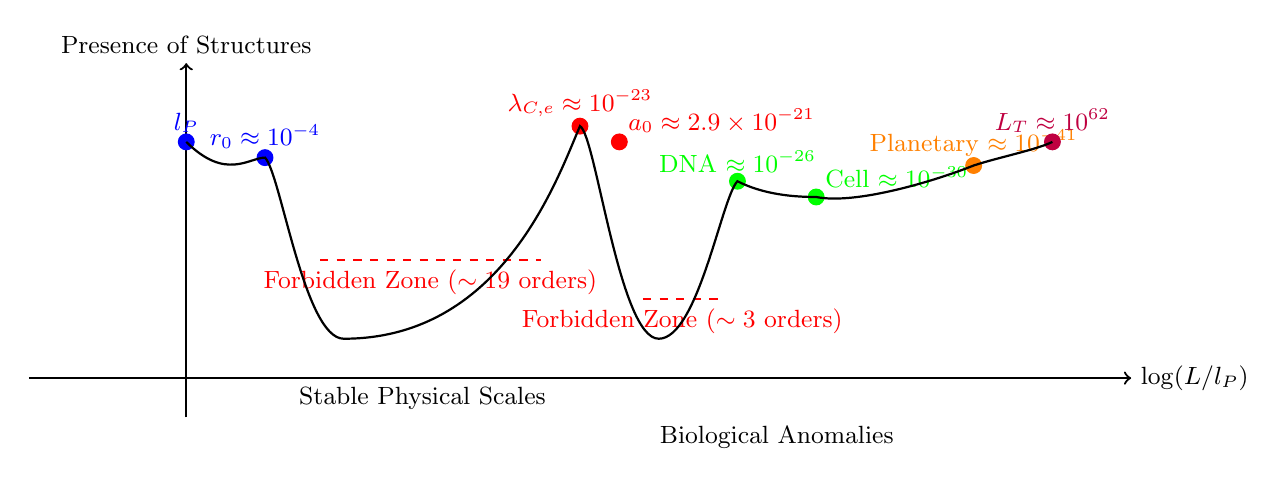
\begin{tikzpicture}
			\small
			\draw[thick,->] (-2,0) -- (12,0) node[right] {$\log(L/l_P)$};
			\draw[thick,->] (0,-0.5) -- (0,4) node[above] {Presence of Structures};
			\filldraw[blue] (0,3) circle (0.1) node[above] {$l_P$};
			\filldraw[blue] (1,2.8) circle (0.1) node[above] {$r_0 \approx 10^{-4}$};
			\filldraw[red] (5,3.2) circle (0.1) node[above] {$\lambda_{C,e} \approx 10^{-23}$};
			\filldraw[red] (5.5,3) circle (0.1) node[above right] {$a_0 \approx 2.9 \times 10^{-21}$};
			\filldraw[green] (7,2.5) circle (0.1) node[above] {DNA $\approx 10^{-26}$};
			\filldraw[green] (8,2.3) circle (0.1) node[above right] {Cell $\approx 10^{-30}$};
			\filldraw[orange] (10,2.7) circle (0.1) node[above] {Planetary $\approx 10^{-41}$};
			\filldraw[purple] (11,3) circle (0.1) node[above] {$L_T \approx 10^{62}$};
			\draw[thick, dashed, red] (1.7,1.5) -- (4.5,1.5) node[midway, below] {Forbidden Zone ($\sim 19$ orders)};
			\draw[thick, dashed, red] (5.8,1) -- (6.8,1) node[midway, below] {Forbidden Zone ($\sim 3$ orders)};
			\draw[smooth, thick] (0,3) .. controls (0.5,2.5) and (0.8,2.8) .. (1,2.8)
			.. controls (1.2,2.6) and (1.5,0.5) .. (2,0.5)
			.. controls (4,0.5) and (4.7,2.5) .. (5,3.2)
			.. controls (5.2,3.1) and (5.5,0.5) .. (6,0.5)
			.. controls (6.5,0.5) and (6.8,2.3) .. (7,2.5)
			.. controls (7.2,2.4) and (7.5,2.3) .. (8,2.3)
			.. controls (8.5,2.2) and (9.5,2.5) .. (10,2.7)
			.. controls (10.3,2.8) and (10.8,2.9) .. (11,3);
			\node[align=center, below] at (3,0) {Stable Physical Scales};
			\node[align=center, below] at (7.5,-0.5) {Biological Anomalies};
		\end{tikzpicture}
		\caption{Stability Centers and Forbidden Zones in the T0 Model’s Length Scale Hierarchy, highlighting biological anomalies (DNA at \(\sim 10^{-26} l_P\), Cell at \(\sim 10^{-30} l_P\)). The forbidden zones, spanning ~19 and ~3 orders of magnitude, are explained in Section \ref{sec:bio_anomalies}. Note: Schematic scaling compresses \(\log(L/l_P)\) for readability; actual positions are DNA at \(\log(10^{-26}) = -26\), Cell at \(\log(10^{-30}) = -30\). Linked to Table \ref{tab:bio_anomalies}, referenced in Section \ref{subsec:quantization}, and discussed in Section \ref{sec:bio_anomalies}.}
		\label{fig:stability_zones}
	\end{figure}
	
	Forbidden zones, spanning orders of magnitude, are stabilized for biological structures (Section \ref{sec:bio_anomalies}). The quantization resembles:
	\begin{itemize}
		\item \textbf{Atomic Orbitals}: Discrete energy levels, as visualized in Figure \ref{fig:orbital_analogy}.
		\item \textbf{Band Gaps}: Forbidden energy zones in solids.
		\item \textbf{Resonances}: Harmonic system frequencies \cite{pascher_quantum_2025}.
	\end{itemize}
	
	\begin{figure}[htbp]
		\centering
		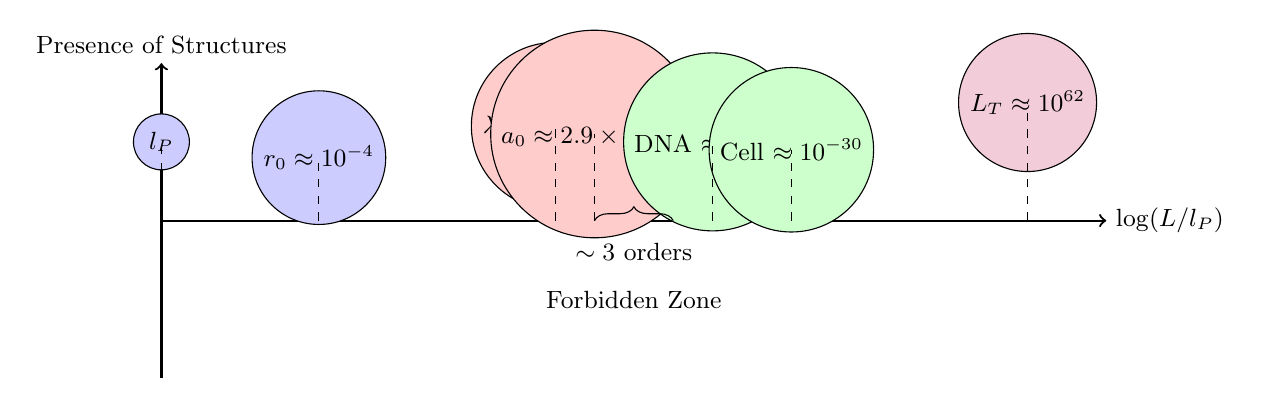
\begin{tikzpicture}
			\small
			\draw[thick,->] (0,0) -- (12,0) node[right] {$\log(L/l_P)$};
			\draw[thick,->] (0,-2) -- (0,2) node[above] {Presence of Structures};
			\node at (0,1) [circle, draw, fill=blue!20] {$l_P$};
			\node at (2,0.8) [circle, draw, fill=blue!20] {$r_0 \approx 10^{-4}$};
			\node at (5,1.2) [circle, draw, fill=red!20] {$\lambda_{C,e} \approx 10^{-23}$};
			\node at (5.5,1.1) [circle, draw, fill=red!20] {$a_0 \approx 2.9 \times 10^{-21}$};
			\node at (7,1) [circle, draw, fill=green!20] {DNA $\approx 10^{-26}$};
			\node at (8,0.9) [circle, draw, fill=green!20] {Cell $\approx 10^{-30}$};
			\node at (11,1.5) [circle, draw, fill=purple!20] {$L_T \approx 10^{62}$};
			\draw[dashed] (0,0) -- (0,1);
			\draw[dashed] (2,0) -- (2,0.8);
			\draw[dashed] (5,0) -- (5,1.2);
			\draw[dashed] (5.5,0) -- (5.5,1.1);
			\draw[dashed] (7,0) -- (7,1);
			\draw[dashed] (8,0) -- (8,0.9);
			\draw[dashed] (11,0) -- (11,1.5);
			\node at (6,-1) {Forbidden Zone};
			\draw[decorate,decoration={brace,amplitude=5pt}] (5.5,0) -- (6.5,0) node[midway,below,yshift=-5pt] {$\sim 3$ orders};
		\end{tikzpicture}
		\caption{Analogy to atomic orbitals, showing discrete scales and forbidden zones with biological anomalies (DNA at \(\sim 10^{-26} l_P\), Cell at \(\sim 10^{-30} l_P\)) in the T0 model. Note: Schematic scaling compresses \(\log(L/l_P)\); actual positions are DNA at \(\log(10^{-26}) = -26\), Cell at \(\log(10^{-30}) = -30\). Linked to Table \ref{tab:bio_anomalies} and Section \ref{subsec:quantization}.}
		\label{fig:orbital_analogy}
	\end{figure}
	
	Empirical validations include:
	\begin{itemize}
		\item \textbf{Subatomic}: Particle sizes match predicted scales.
		\item \textbf{Atomic}: Bohr radius clustering.
		\item \textbf{Biological}: DNA and cells in forbidden zones (Section \ref{sec:bio_anomalies}).
		\item \textbf{Cosmic}: Galaxy size concentrations \cite{pascher_galaxies_2025}.
	\end{itemize}
	
	Testable predictions are:
	\begin{itemize}
		\item No stable particles in forbidden zones.
		\item Galaxy size clustering, as shown in Figure \ref{fig:stability_zones}.
		\item Resonance phenomena at quantized scales \cite{pascher_quantum_2025}.
	\end{itemize}
	
	Philosophically, this suggests:
	\begin{enumerate}
		\item \textbf{Ontological Discreteness}: Reality is layered, not continuous.
		\item \textbf{Emergent Complexity}: New phenomena at each scale.
		\item \textbf{Cross-Scale Unity}: Constants like \(\xi\) connect levels.
		\item \textbf{Deterministic Structure}: A cosmic order, akin to a “periodic table of scales” \cite{pascher_perspective_2025}.
	\end{enumerate}
	
	\subsection{Einstein-Hilbert Action and Emergent Gravitation}
	\label{sec:gravitation}
	
	The T0 model reinterprets gravitation via the Einstein-Hilbert action:
	\[
	S_{\text{EH}} = \frac{1}{16 \pi} \int (R - 2 \kappa) \sqrt{-g} \, d^4x
	\]
	The modified potential:
	\[
	\Phi(r) = -\frac{M}{r} + \kappa r
	\]
	with \(\kappa \approx \SI{4.8e-11}{\meter\per\second\squared}\), explains dark energy naturally, as linked to \(\Lambda_{\text{eff}} = \kappa\). Gravitation emerges from:
	\[
	\Phi(\vec{x}) = -\ln\left(\frac{\Tfield}{\Tfield_0}\right)
	\]
	This unifies quantum and cosmic scales, as shown in Table \ref{tab:theory_comparison} \cite{pascher_emergente_2025}.
	
	\begin{table}[htbp]
		\centering
		\begin{adjustbox}{width=\tablescale\textwidth}
			\begin{tabular}{p{3cm}p{3cm}p{4cm}p{4cm}}
				\toprule
				\textbf{Theory} & \textbf{Principle} & \textbf{Potential} & \textbf{Comparison with T0} \\
				\midrule
				Newtonian & Force & \(-\frac{G M}{r}\) & T0 special case (\(\kappa = 0\)) \\
				General Relativity & Curvature & Schwarzschild & Equivalent in weak fields \\
				MOND & Modified dynamics & \(\mu(\nabla \Phi/a_0)\) & T0 provides basis \\
				f(R) Theories & Modified action & Varies & T0: f(R) = R - 2\(\kappa\) G \\
				T0 Model & Time field & \(-\frac{M}{r} + \kappa r\) & Unifies QM and gravitation \\
				\bottomrule
			\end{tabular}
		\end{adjustbox}
		\caption{Comparison of Gravitation Theories, linked to Section \ref{subsec:t0_equations}}
		\label{tab:theory_comparison}
	\end{table}
	
	\subsection{Field Equations}
	\label{sec:field_equations}
	
	\subsubsection{Maxwell Equations}
	\label{subsec:maxwell}
	
	With \(\alphaEM = 1\), \(\varepsilon_0 = \mu_0 = 1\), Maxwell’s equations simplify, as shown in Table \ref{tab:maxwell}. The dimensionless charge \(e = \sqrt{4\pi}\) unifies field dimensions, as discussed in Section \ref{subsec:alpha_derivation} \cite{pascher_alpha_2025}.
	
	\begin{table}[htbp]
		\centering
		\begin{adjustbox}{width=\tablescale\textwidth}
			\begin{tabular}{llll}
				\toprule
				\textbf{Equation} & \textbf{Classical Form} & \textbf{Natural Form} & \textbf{Simplification} \\
				\midrule
				Gauss’s Law & \(\nabla \cdot \vec{E} = \frac{\rho}{\varepsilon_0}\) & \(\nabla \cdot \vec{E} = \rho\) & Direct source \\
				Ampère’s Law & \(\nabla \times \vec{B} - \mu_0 \varepsilon_0 \frac{\partial \vec{E}}{\partial t} = \mu_0 \vec{j}\) & \(\nabla \times \vec{B} - \frac{\partial \vec{E}}{\partial t} = \vec{j}\) & Direct source \\
				Gauss for Magnetism & \(\nabla \cdot \vec{B} = 0\) & \(\nabla \cdot \vec{B} = 0\) & Unchanged \\
				Faraday’s Law & \(\nabla \times \vec{E} + \frac{\partial \vec{B}}{\partial t} = 0\) & \(\nabla \times \vec{E} + \frac{\partial \vec{B}}{\partial t} = 0\) & Unchanged \\
				\bottomrule
			\end{tabular}
		\end{adjustbox}
		\caption{Maxwell Equations in Natural Units, linked to Table \ref{tab:em_const}}
		\label{tab:maxwell}
	\end{table}
	
	\subsubsection{T0 Model Equations}
	\label{subsec:t0_equations}
	
	The T0 model’s equations, shown in Table \ref{tab:t0_equations}, reflect emergent gravitation and cosmic dynamics, as linked to Section \ref{sec:gravitation} \cite{pascher_emergente_2025}.
	
	\begin{table}[htbp]
		\centering
		\begin{adjustbox}{width=\tablescale\textwidth}
			\begin{tabular}{lll}
				\toprule
				\textbf{Equation} & \textbf{Natural Form} & \textbf{Significance} \\
				\midrule
				Temperature-Redshift & \(T(z) = T_0 (1+z)(1+\ln(1+z))\) & Cosmic temperature \\
				Wavelength Redshift & \(z(\lambda) = z_0 (1+\ln(\lambda/\lambda_0))\) & Frequency-dependent \\
				Gravitational Potential & \(\Phi(r) = -\frac{M}{r} + r\) & Emergent gravitation \\
				Intrinsic Time Field & \(\nabla^2 \Tfield \approx -\frac{\rho}{\Tfield^2}\) & Source term \\
				Effective Potential & \(\Phi(\vec{x}) = -\ln\left(\frac{\Tfield}{\Tfield_0}\right)\) & Gravitation link \\
				Gravitational Force & \(\vec{F} = -\frac{\nabla \Tfield}{\Tfield}\) & Force from time field \\
				\bottomrule
			\end{tabular}
		\end{adjustbox}
		\caption{T0 Model Equations, linked to Section \ref{sec:gravitation}}
		\label{tab:t0_equations}
	\end{table}
	
	\subsubsection{Modified Quantum Mechanics}
	\label{subsec:quantum}
	
	The Ttx model modifies quantum mechanics via \(\Tfield\), as shown in Table \ref{tab:qm_equations}. The Schrödinger equation:
	\[
	i \Tfield \frac{\partial \Psi}{\partial t} + i \Psi \frac{\partial \Tfield}{\partial t} = \hat{H} \Psi
	\]
	introduces mass-dependent dynamics, explaining decoherence and nonlocality, as visualized in Figure \ref{fig:orbital_analogy} \cite{pascher_quantum_2025}.
	
	\begin{table}[htbp]
		\centering
		\begin{adjustbox}{width=\tablescale\textwidth}
			\begin{tabular}{lll}
				\toprule
				\textbf{Equation} & \textbf{Natural Form} & \textbf{Standard Form} \\
				\midrule
				Schrödinger Equation & \(i \Tfield \frac{\partial \Psi}{\partial t} + i \Psi \frac{\partial \Tfield}{\partial t} = \hat{H} \Psi\) & \(i \hbar \frac{\partial \Psi}{\partial t} = \hat{H} \Psi\) \\
				Decoherence Rate & \(\Gamma_{\text{dec}} = \Gamma_0 \cdot m\) & \(\Gamma_{\text{dec}} = \Gamma_0 \cdot \frac{m c^2}{\hbar}\) \\
				Wave-Particle & \(\lambda = \frac{1}{p}\) & \(\lambda = \frac{h}{p}\) \\
				Uncertainty & \(\Delta E \cdot \Delta t \geq \frac{1}{2}\) & \(\Delta E \cdot \Delta t \geq \frac{\hbar}{2}\) \\
				\bottomrule
			\end{tabular}
		\end{adjustbox}
		\caption{Modified Quantum Equations, linked to Figure \ref{fig:orbital_analogy}}
		\label{tab:qm_equations}
	\end{table}
	
	\subsection{Fundamental Relationships}
	\label{subsec:relationships}
	
	The T0 model’s quantities form a network, as shown in Figure \ref{fig:quantity_network}, linked to scales in Figure \ref{fig:energy_hierarchy} \cite{pascher_grundkraefte_2025}.
	
	\begin{figure}[htbp]
		\centering
		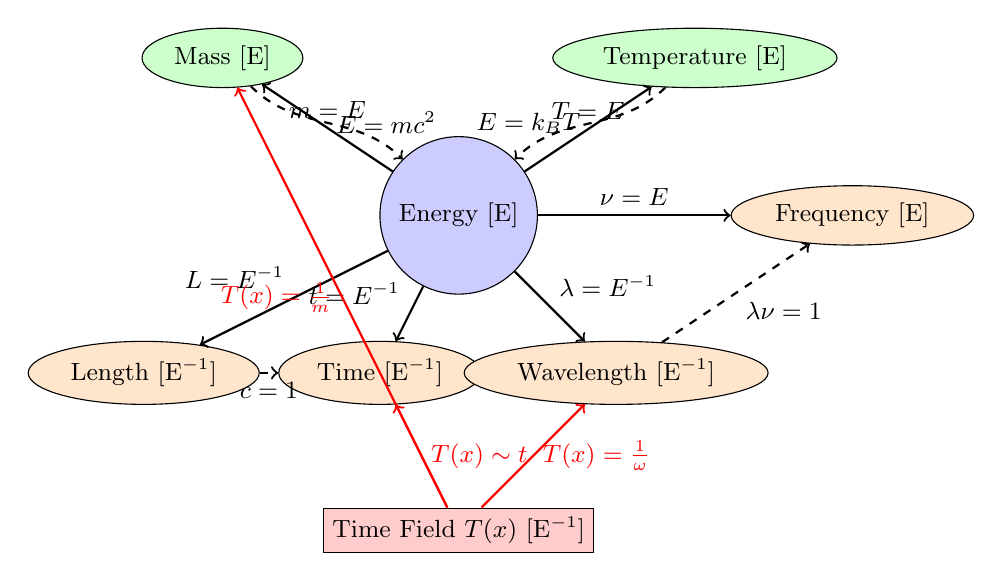
\begin{tikzpicture}
			\small
			\node[draw, circle, fill=blue!20, minimum size=2cm] (energy) at (0,0) {Energy [E]};
			\node[draw, ellipse, fill=green!20] (mass) at (-3,2) {Mass [E]};
			\node[draw, ellipse, fill=green!20] (temp) at (3,2) {Temperature [E]};
			\node[draw, ellipse, fill=orange!20] (length) at (-4,-2) {Length [E\(^{-1}\)]};
			\node[draw, ellipse, fill=orange!20] (time) at (-1,-2) {Time [E\(^{-1}\)]};
			\node[draw, ellipse, fill=orange!20] (wavelength) at (2,-2) {Wavelength [E\(^{-1}\)]};
			\node[draw, ellipse, fill=orange!20] (frequency) at (5,0) {Frequency [E]};
			\node[draw, rectangle, fill=red!20] (tfield) at (0,-4) {Time Field \(\Tfield\) [E\(^{-1}\)]};
			\draw[->, thick] (energy) -- (mass) node[midway, above] {$m = E$};
			\draw[->, thick] (energy) -- (temp) node[midway, above] {$T = E$};
			\draw[->, thick] (energy) -- (length) node[midway, above left] {$L = E^{-1}$};
			\draw[->, thick] (energy) -- (time) node[midway, above left] {$t = E^{-1}$};
			\draw[->, thick] (energy) -- (wavelength) node[midway, above right] {$\lambda = E^{-1}$};
			\draw[->, thick] (energy) -- (frequency) node[midway, above] {$\nu = E$};
			\draw[->, thick, dashed] (length) -- (time) node[midway, below] {$c = 1$};
			\draw[->, thick, dashed] (wavelength) -- (frequency) node[midway, below right] {$\lambda \nu = 1$};
			\draw[->, thick, dashed] (mass) to[out=-45, in=135] node[midway, right] {$E = m c^2$} (energy);
			\draw[->, thick, dashed] (temp) to[out=-135, in=45] node[midway, left] {$E = k_B T$} (energy);
			\draw[->, thick, red] (tfield) -- (mass) node[midway, left] {$\Tfield = \frac{1}{m}$};
			\draw[->, thick, red] (tfield) -- (time) node[midway, right] {$\Tfield \sim t$};
			\draw[->, thick, red] (tfield) -- (wavelength) node[midway, right] {$\Tfield = \frac{1}{\omega}$};
		\end{tikzpicture}
		\caption{Network of physical quantities, linked to Table \ref{tab:practical_notation}}
		\label{fig:quantity_network}
	\end{figure}
	
	\begin{figure}[htbp]
		\centering
		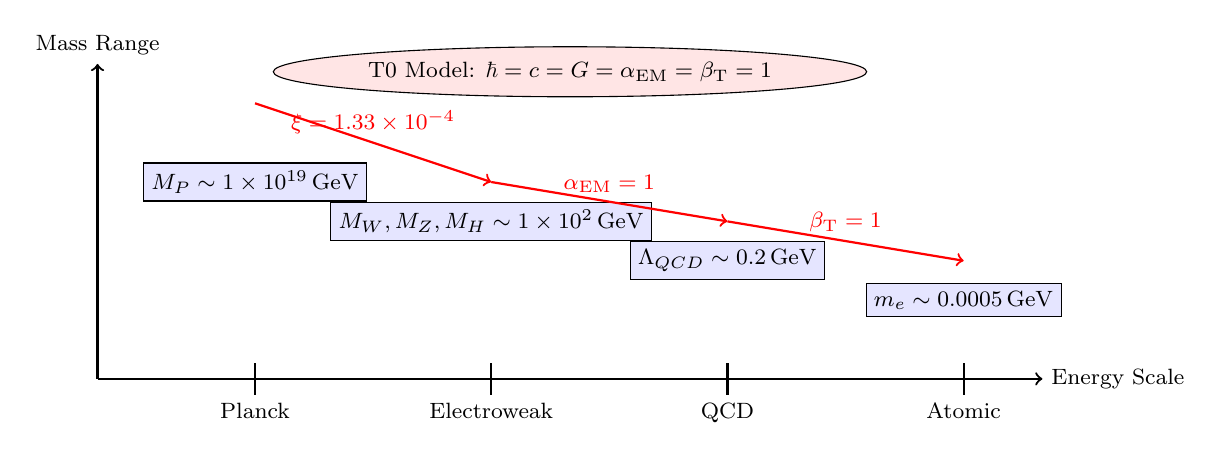
\begin{tikzpicture}
			\footnotesize
			\draw[thick, ->] (0,0) -- (12,0) node[right] {Energy Scale};
			\draw[thick, ->] (0,0) -- (0,4) node[above] {Mass Range};
			\draw[thick] (2,0.2) -- (2,-0.2) node[below] {Planck};
			\draw[thick] (5,0.2) -- (5,-0.2) node[below] {Electroweak};
			\draw[thick] (8,0.2) -- (8,-0.2) node[below] {QCD};
			\draw[thick] (11,0.2) -- (11,-0.2) node[below] {Atomic};
			\node[draw, fill=blue!10] at (2,2.5) {$M_P \sim \SI{1e19}{\giga\electronvolt}$};
			\node[draw, fill=blue!10] at (5,2) {$M_W, M_Z, M_H \sim \SI{1e2}{\giga\electronvolt}$};
			\node[draw, fill=blue!10] at (8,1.5) {$\Lambda_{QCD} \sim \SI{0.2}{\giga\electronvolt}$};
			\node[draw, fill=blue!10] at (11,1) {$m_e \sim \SI{0.0005}{\giga\electronvolt}$};
			\draw[thick, red, ->] (2,3.5) -- (5,2.5) node[midway, above] {$\xi = 1.33 \times 10^{-4}$};
			\draw[thick, red, ->] (5,2.5) -- (8,2) node[midway, above] {$\alphaEM = 1$};
			\draw[thick, red, ->] (8,2) -- (11,1.5) node[midway, above] {$\betaT = 1$};
			\node[draw, ellipse, fill=red!10] at (6,3.9) {T0 Model: $\hbar = c = G = \alphaEM = \betaT = 1$};
		\end{tikzpicture}
		\caption{Energy scale hierarchy, linked to Section \ref{subsec:higgs}}
		\label{fig:energy_hierarchy}
	\end{figure}
	
	
	%------
	\subsection{Fundamental Forces}
	\label{subsec:forces}
	
	The T0 model reinterprets forces, as shown in Table \ref{tab:forces}, with gravitation emergent from \(\Tfield\) (Section \ref{sec:gravitation}) \cite{pascher_grundkraefte_2025}.
	
	\begin{table}[htbp]
		\centering
		\begin{adjustbox}{width=\tablescale\textwidth}
			\begin{tabular}{llll}
				\toprule
				\textbf{Force} & \textbf{Dimensionless Coupling} & \textbf{Natural Value} & \textbf{Range} \\
				\midrule
				Electromagnetic & \(\alphaEM\) & 1 & \(\infty\) \\
				Strong & \(\alpha_s\) & \(\sim 0.118\) at \(Q^2 = M_Z^2\) & \(\sim \SI{1e-15}{\meter}\) \\
				Weak & \(\alpha_W = g^2/(4\pi)\) & \(\sim 1/30\) & \(\sim \SI{1e-18}{\meter}\) \\
				Gravitation & \(\alpha_G = G m^2/\hbar c\) & \(m^2/m_P^2\) & \(\infty\) \\
				\bottomrule
			\end{tabular}
		\end{adjustbox}
		\caption{Fundamental Forces in Natural Units, linked to Section \ref{subsec:maxwell}}
		\label{tab:forces}
	\end{table}
	
	\subsection{Unit Conversions}
	\label{sec:conversions}
	
	Conversions to SI units are precise, as shown in Table \ref{tab:conversion}, linked to Figure \ref{fig:practical_conversion} \cite{pascher_temp_2025}.
	
	\begin{table}[htbp]
		\centering
		\begin{adjustbox}{width=\tablescale\textwidth}
			\begin{tabular}{lcccc}
				\toprule
				\textbf{SI Unit} & \textbf{SI Dimension} & \textbf{T0 Equivalent} & \textbf{Conversion} & \textbf{Accuracy} \\
				\midrule
				Meter & \([L]\) & \([E^{-1}]\) & \(\SI{1}{\meter} \leftrightarrow (\SI{197}{\mega\electronvolt})^{-1}\) & \(< 0.001\%\) \\
				Second & \([T]\) & \([E^{-1}]\) & \(\SI{1}{\second} \leftrightarrow (\SI{6.58e-22}{\mega\electronvolt})^{-1}\) & \(< 0.00001\%\) \\
				Kilogram & \([M]\) & \([E]\) & \(\SI{1}{\kilogram} \leftrightarrow \SI{5.61e26}{\mega\electronvolt}\) & \(< 0.001\%\) \\
				Ampere & \([I]\) & \([E]\) & \(\SI{1}{\ampere} \leftrightarrow [E^2]\) & \(< 0.005\%\) \\
				Kelvin & \([\Theta]\) & \([E]\) & \(\SI{1}{\kelvin} \leftrightarrow \SI{8.62e-5}{\electronvolt}\) & \(< 0.01\%\) \\
				Volt & \([ML^2 T^{-3} I^{-1}]\) & \([E]\) & \(\SI{1}{\volt} \leftrightarrow \SI{1}{\electronvolt}/\sqrt{4\pi}\) & \(< 0.0001\%\) \\
				Coulomb & \([T I]\) & \([1]\) & \(\SI{1}{\coulomb} \leftrightarrow \sqrt{4\pi}/e\) & \(< 0.0001\%\) \\
				\bottomrule
			\end{tabular}
		\end{adjustbox}
		\caption{Conversion of SI Units to T0 Units, linked to Table \ref{tab:planck_units}}
		\label{tab:conversion}
	\end{table}
	
	\begin{figure}[htbp]
		\centering
		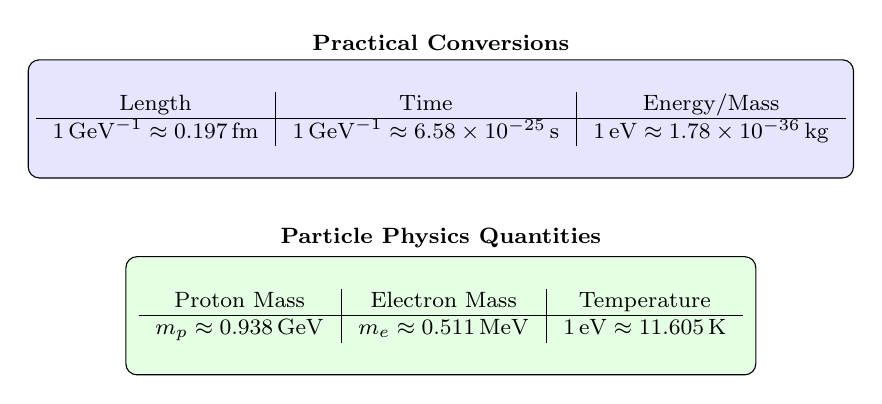
\begin{tikzpicture}
			\footnotesize
			\node[draw, rounded corners, fill=blue!10, minimum width=8cm, minimum height=1.5cm] (conversion) at (0,0) {
				\begin{tabular}{c|c|c}
					Length & Time & Energy/Mass \\
					\hline
					\(\SI{1}{\per\giga\electronvolt} \approx \SI{0.197}{\femto\meter}\) & \(\SI{1}{\per\giga\electronvolt} \approx \SI{6.58e-25}{\second}\) & \(\SI{1}{\electronvolt} \approx \SI{1.78e-36}{\kilogram}\)
				\end{tabular}
			};
			\node[draw, rounded corners, fill=green!10, minimum width=8cm, minimum height=1.5cm] (practical) at (0,-2.5) {
				\begin{tabular}{c|c|c}
					Proton Mass & Electron Mass & Temperature \\
					\hline
					\(m_p \approx \SI{0.938}{\giga\electronvolt}\) & \(m_e \approx \SI{0.511}{\mega\electronvolt}\) & \(\SI{1}{\electronvolt} \approx \SI{11.605}{\kelvin}\)
				\end{tabular}
			};
			\node[above] at (conversion.north) {\textbf{Practical Conversions}};
			\node[above] at (practical.north) {\textbf{Particle Physics Quantities}};
		\end{tikzpicture}
		\caption{Conversions in Natural Units, linked to Section \ref{sec:conversions}}
		\label{fig:practical_conversion}
	\end{figure}
	
	\subsection{Philosophical Implications}
	\label{sec:philosophy}
	
	The T0 model’s energy-based framework carries profound implications:
	\begin{enumerate}
		\item \textbf{Ontological Simplification}: Energy as the sole entity unifies all phenomena, aligning with Einstein’s insights \cite{Einstein1905, pascher_dualismus_2025}.
		\item \textbf{Unified Description}: Normalized constants reveal a singular framework \cite{pascher_vereinheitlichung_2025}.
		\item \textbf{Emergent Space-Time}: Space-time arises from \(\Tfield\), as shown in Figure \ref{fig:quantity_network} \cite{pascher_perspective_2025}.
		\item \textbf{Mind-Body Problem}: Absolute time offers a foundation for consciousness \cite{pascher_perspective_2025}.
	\end{enumerate}
	
	\section{Summary and Outlook}
	\label{sec:outlook}
	
	The T0 model unifies physics with:
	\begin{enumerate}
		\item Hierarchical constants (Section \ref{sec:hierarchy}).
		\item Quantized scales (Section \ref{subsec:quantization}).
		\item Simplified equations (Section \ref{sec:field_equations}).
		\item Emergent gravitation (Section \ref{sec:gravitation}).
		\item Cosmological insights (Section \ref{subsec:t0_equations}) \cite{pascher_alphabeta_2025}.
	\end{enumerate}
	
	Future directions include:
	\begin{itemize}
		\item Testing redshift predictions.
		\item Verifying \(R_\infty = m_e/2\).
		\item Quantizing \(\Tfield\).
		\item Simulating galaxy dynamics \cite{pascher_galaxies_2025}.
	\end{itemize}
	
	\bibliographystyle{apsrev4-2}
	\begin{thebibliography}{99}
		\bibitem{pascher_zeit_2025} J. Pascher, \href{https://github.com/jpascher/T0-Time-Mass-Duality/tree/main/2/pdf/English/ZeitEmergentQMEn.pdf}{Time as an Emergent Property in Quantum Mechanics}, March 23, 2025.
		\bibitem{pascher_messdifferenzen_2025} J. Pascher, \href{https://github.com/jpascher/T0-Time-Mass-Duality/tree/main/2/pdf/English/MessdifferenzenT0StandardEn.pdf}{Compensatory and Additive Effects}, April 2, 2025.
		\bibitem{pascher_galaxies_2025} J. Pascher, \href{https://github.com/jpascher/T0-Time-Mass-Duality/tree/main/2/pdf/English/MassVarGalaxienEn.pdf}{Mass Variation in Galaxies}, March 30, 2025.
		\bibitem{pascher_params_2025} J. Pascher, \href{https://github.com/jpascher/T0-Time-Mass-Duality/tree/main/2/pdf/English/ZeitMasseT0ParamsEn.pdf}{Time-Mass Duality Theory}, March 30, 2025.
		\bibitem{pascher_temp_2025} J. Pascher, \href{https://github.com/jpascher/T0-Time-Mass-Duality/tree/main/2/pdf/English/NatEinheitenAlpha1En.pdf}{Adjustment of Temperature Units}, April 2, 2025.
		\bibitem{pascher_alpha_2025} J. Pascher, \href{https://github.com/jpascher/T0-Time-Mass-Duality/tree/main/2/pdf/English/NatEinheitenAlpha1En.pdf}{Energy as a Fundamental Unit}, March 26, 2025.
		\bibitem{pascher_beta_2025} J. Pascher, \href{https://github.com/jpascher/T0-Time-Mass-Duality/tree/main/2/pdf/English/Alpha1Beta1KonsistenzEn.pdf}{Dimensionless Parameters}, April 4, 2025.
		\bibitem{pascher_higgs_2025} J. Pascher, \href{https://github.com/jpascher/T0-Time-Mass-Duality/tree/main/2/pdf/English/MathHiggsZeitMasseEn.pdf}{Higgs Mechanism}, March 28, 2025.
		\bibitem{pascher_lagrange_2025} J. Pascher, \href{https://github.com/jpascher/T0-Time-Mass-Duality/tree/main/2/pdf/English/MathZeitMasseLagrangeEn.pdf}{From Time Dilation to Mass Variation}, March 29, 2025.
		\bibitem{pascher_emergente_2025} J. Pascher, \href{https://github.com/jpascher/T0-Time-Mass-Duality/tree/main/2/pdf/English/EmergentGravT0En.pdf}{Emergent Gravitation}, April 1, 2025.
		\bibitem{pascher_perspective_2025} J. Pascher, \href{https://github.com/jpascher/T0-Time-Mass-Duality/tree/main/2/pdf/English/ZeitRaumPascherEn.pdf}{A New Perspective on Time and Space}, March 25, 2025.
		\bibitem{pascher_dualismus_2025} J. Pascher, \href{https://github.com/jpascher/T0-Time-Mass-Duality/tree/main/2/pdf/English/KurzKomplementDualPhysikEn.pdf}{Complementary Duality}, March 26, 2025.
		\bibitem{pascher_grundkraefte_2025} J. Pascher, \href{https://github.com/jpascher/T0-Time-Mass-Duality/tree/main/2/pdf/English/VierKraefteZeitMasseEn.pdf}{Fundamental Forces}, March 27, 2025.
		\bibitem{pascher_zeit_masse_2025} J. Pascher, \href{https://github.com/jpascher/T0-Time-Mass-Duality/tree/main/2/pdf/English/ZeitMasseNeuerBlickEn.pdf}{Time and Mass}, March 22, 2025.
		\bibitem{pascher_quantum_2025} J. Pascher, \href{https://github.com/jpascher/T0-Time-Mass-Duality/tree/main/2/pdf/English/NotwendigkeitQMErweiterungEn.pdf}{Extending Quantum Mechanics}, March 27, 2025.
		\bibitem{pascher_photons_2025} J. Pascher, \href{https://github.com/jpascher/T0-Time-Mass-Duality/tree/main/2/pdf/English/DynMassePhotonenNichtlokalEn.pdf}{Dynamic Mass of Photons}, March 25, 2025.
		\bibitem{pascher_alphabeta_2025} J. Pascher, \href{https://github.com/jpascher/T0-Time-Mass-Duality/tree/main/2/pdf/English/Alpha1Beta1KonsistenzEn.pdf}{Unified Unit System}, April 5, 2025.
		\bibitem{pascher_planck_2025} J. Pascher, \href{https://github.com/jpascher/T0-Time-Mass-Duality/tree/main/2/pdf/English/JenseitsPlanckEn.pdf}{Beyond the Planck Scale}, March 24, 2025.
		\bibitem{pascher_energiedynamik_2025} J. Pascher, \href{https://github.com/jpascher/T0-Time-Mass-Duality/tree/main/2/pdf/English/MathEnergiedynamikEn.pdf}{Dark Energy}, April 3, 2025.
		\bibitem{pascher_vereinheitlichung_2025} J. Pascher, \href{https://github.com/jpascher/T0-Time-Mass-Duality/tree/main/2/pdf/English/T0VereinheitlichungDEGalEn.pdf}{Unification of the T0 Model}, April 4, 2025.
		\bibitem{pascher_formalismen_2025} J. Pascher, \href{https://github.com/jpascher/T0-Time-Mass-Duality/tree/main/2/pdf/English/MathZeitMasseLagrangeEn.pdf}{Mathematical Core Formulations}, April 5, 2025.
		\bibitem{Planck1899} M. Planck, \textit{On Irreversible Radiation Processes}, Proc. Roy. Prussian Acad. Sci. 5, 440--480 (1899).
		\bibitem{Dirac1928} P. A. M. Dirac, \textit{The Quantum Theory of the Electron}, Proc. Roy. Soc. London A 117, 610--624 (1928).
		\bibitem{Einstein1905} A. Einstein, \textit{On the Electrodynamics of Moving Bodies}, Ann. Phys. 322, 891--921 (1905).
		\bibitem{Einstein1915} A. Einstein, \textit{The Field Equations of Gravitation}, Proc. Roy. Prussian Acad. Sci., 844--847 (1915).
		\bibitem{Sommerfeld1916} A. Sommerfeld, \textit{On the Quantum Theory of Spectral Lines}, Ann. Phys. 356, 1--94 (1916).
		\bibitem{Heisenberg1927} W. Heisenberg, \textit{On the Perceptual Content}, Z. Phys. 43, 172--198 (1927).
		\bibitem{Schrodinger1926} E. Schrödinger, \textit{Quantization as an Eigenvalue Problem}, Ann. Phys. 384, 361--376 (1926).
		\bibitem{Feynman1985} R. P. Feynman, \textit{QED: The Strange Theory of Light and Matter}, Princeton Univ. Press (1985).
		\bibitem{Duff2002} M. J. Duff et al., \textit{Trialogue on Fundamental Constants}, J. High Energy Phys. 3, 023 (2002).
		\bibitem{Wilczek2008} F. Wilczek, \textit{The Lightness of Being}, Basic Books (2008).
		\bibitem{Verlinde2011} E. Verlinde, \textit{On the Origin of Gravity}, J. High Energy Phys. 4, 29 (2011).
		\bibitem{Greene2020} B. Greene, \textit{Until the End of Time}, Alfred A. Knopf (2020).
		\bibitem{tHooft1993} G. 't Hooft, \textit{Dimensional Reduction}, arXiv:gr-qc/9310026 (1993).
		\bibitem{Will2014} C. M. Will, \textit{General Relativity and Experiment}, Living Rev. Rel. 17, 4 (2014).
	\end{thebibliography}
	
\end{document}		